%MÁSTER UNIVERSITARIO EN GESTIÓN SOSTENIBLE DE LA TIERRA Y EL TERRITORIO
%TÉCNICAS DE ANÁLISIS CUANTITATIVAS Y CUALITATIVAS
%DOCUMENTO DE RESOLUCIÓN DEL EJERCICIO 4 DE EVALUACIÓN
%MARCOS RIAL DOCAMPO


\documentclass[11pt,a4paper]{article}

\usepackage[utf8]{inputenc}
\usepackage[spanish]{babel}
\usepackage{amsmath}
\usepackage{amsfonts}
\usepackage{amssymb}
\usepackage{url}
\usepackage[colorlinks,linktocpage=true,citecolor=blue,linkcolor=blue]{hyperref}
\usepackage{booktabs}
\usepackage{graphicx,geometry}
\usepackage{caption}
\usepackage{verbatim,moreverb}

\usepackage{listings}
\lstset{
	frame=tb,
    framerule=0pt,
    aboveskip=3mm,
    belowskip=3mm,
    framextopmargin=3pt,
    framexbottommargin=3pt,
    %framexleftmargin=0.2cm,
    framesep=0pt,
    rulesep=.4pt,
    backgroundcolor=\color{gray97},
    rulesepcolor=\color{black},
    stringstyle=\color{mauve},
    showstringspaces = false,
    basicstyle=\footnotesize\ttfamily,
    commentstyle=\color{dkgreen},
    keywordstyle=\color{blue},
    numbers=left,
    numbersep=-6.5pt,
    numberstyle=\tiny\color{gray},
    numberfirstline = false,
    breaklines=true,
    morekeywords={*,...}
   }

\usepackage{xcolor}
\definecolor{gray97}{gray}{.97}
\definecolor{gray75}{gray}{.75}
\definecolor{gray45}{gray}{.45}
\definecolor{mauve}{rgb}{0.58,0,0.82}
\definecolor{dkgreen}{rgb}{0,0.6,0}

\author{Marcos Rial Docampo}
\title{Técnicas de Análisis Cuantitativas y Cualitativas\\Resolución del ejercicio de evaluación 4}
\date{\small{\today}}

\begin{document}
\maketitle

Disponemos de datos de los tiempos obtenidos por los participantes de una carrera popular. Se trata de 80 muestras de un total de 1140 que están estratificadas por sexo y categoría de edad.

Mediante un test de Shapiro-Wilk comprobamos si la variable \textit{total.minutos} tiene una distribución normal. Para ello podemos aplicar el test a todas las observaciones de la variable o dividirla en grupos. En este caso dividiremos la variable en los siente grupos correspondientes a la categoría de la prueba, pero podríamos haberlo hecho por sexo o por subcategoría. Obtenemos los resultados mostrados en el cuadro \ref{tab:Shapiro} y los gráficos de la figura \ref{fig:diagrama}.

\begin{table}[ht]
\centering
\begin{tabular}{cr@{,}lr@{,}l}
\toprule[0.4mm]
\multicolumn{5}{c}{Test Shapiro-Wilk}\\
 & \multicolumn{2}{c}{W} & \multicolumn{2}{c}{p-valor}\\
\midrule
Infantil-Cadete & 0&93455 & 0&1888\\
Junior & 0&93301 & 0&1765\\
Senior & 0&96890 & 0&7315\\
Veterano & 0&96757 & 0&7029\\
\bottomrule[0.4mm]
\end{tabular}
\captionsetup{font={footnotesize,it}}
\caption{Resultado del test de Shapiro-Wilk para la variable ``total.minutos''.}
\label{tab:Shapiro}
\end{table}

\begin{figure}
\centering
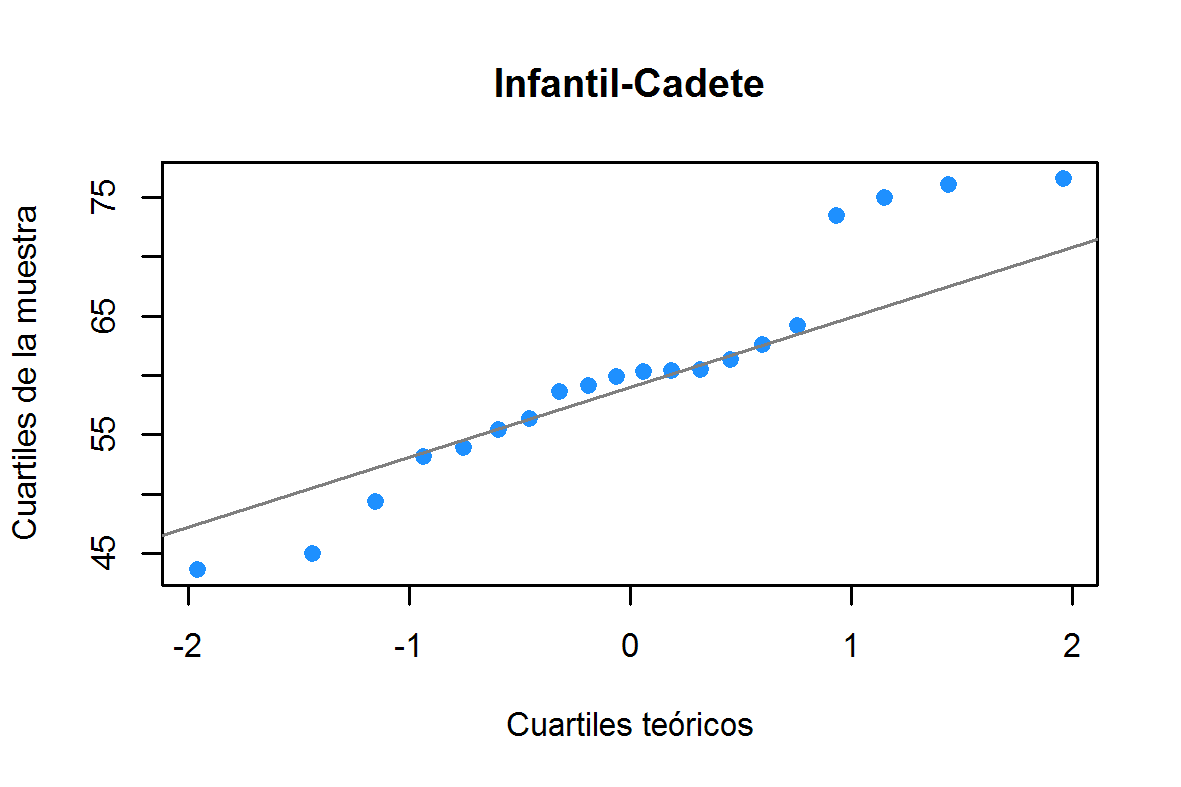
\includegraphics[scale=0.725]{./R/Graficos/CuartInfantil.png}
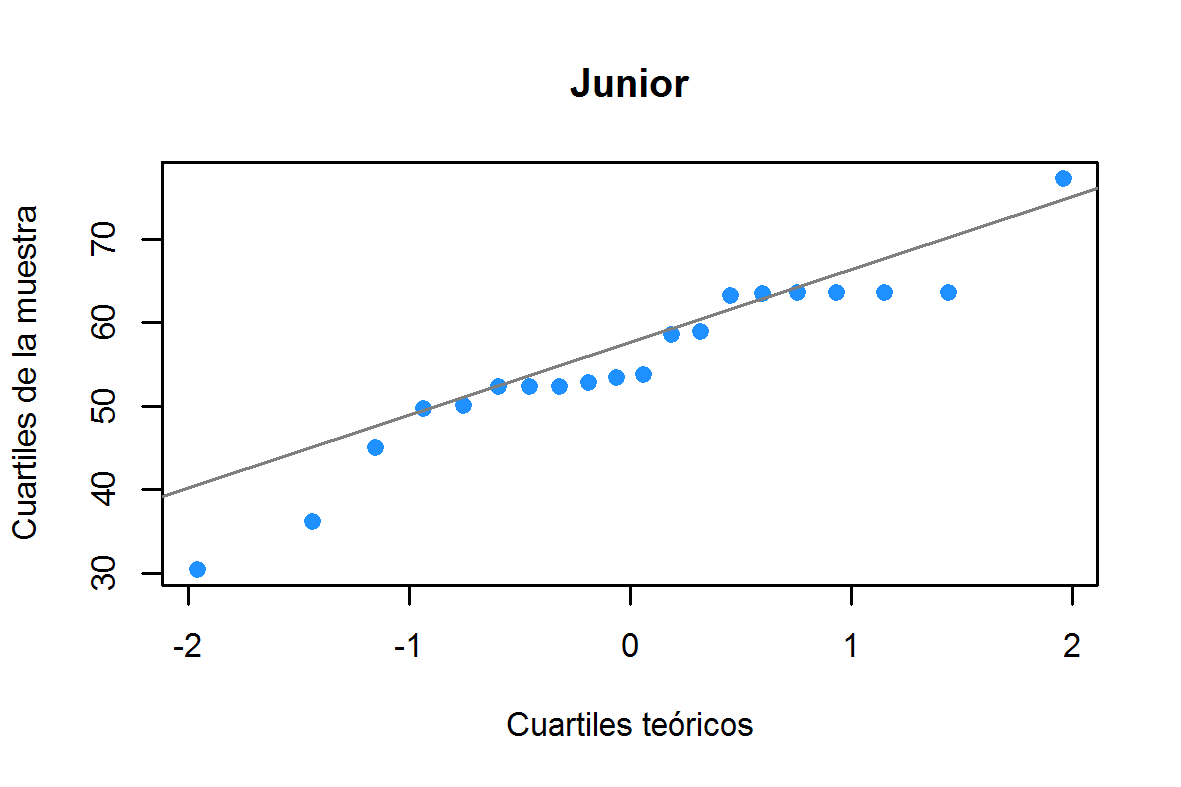
\includegraphics[scale=0.725]{./R/Graficos/CuartJunior.png}
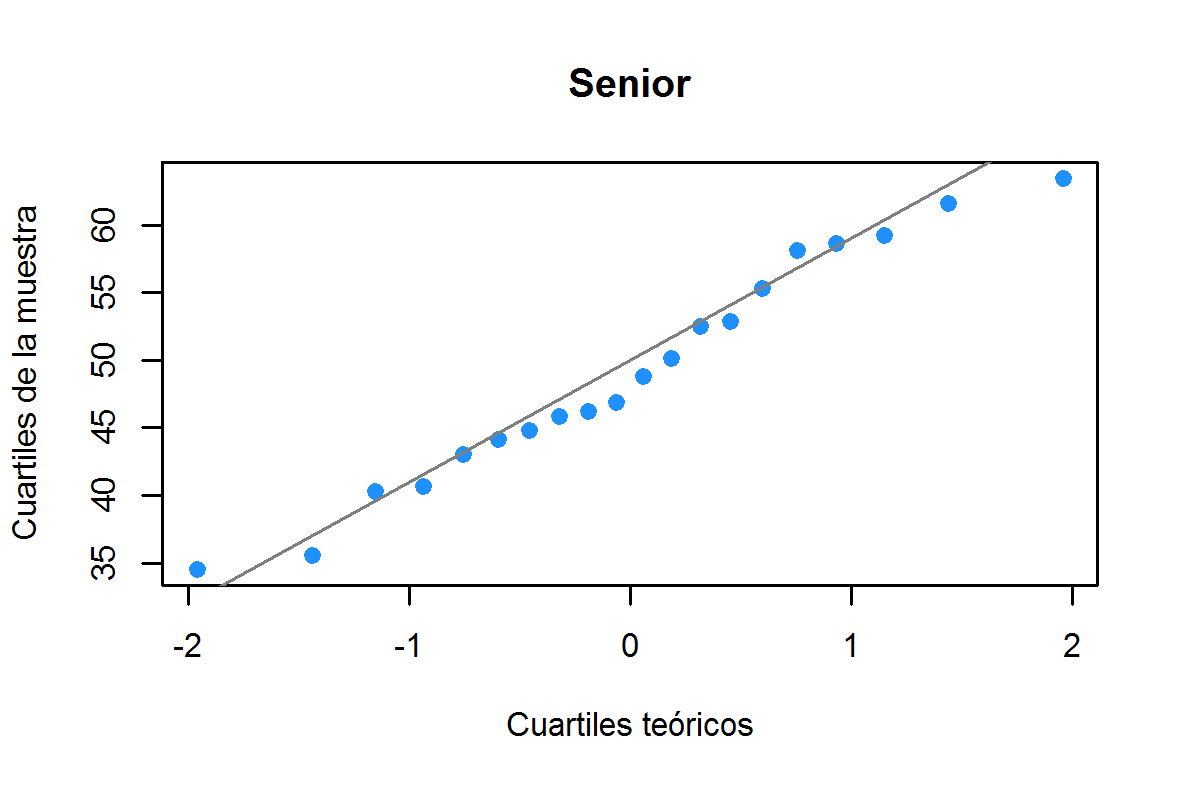
\includegraphics[scale=0.725]{./R/Graficos/CuartSenior.png}
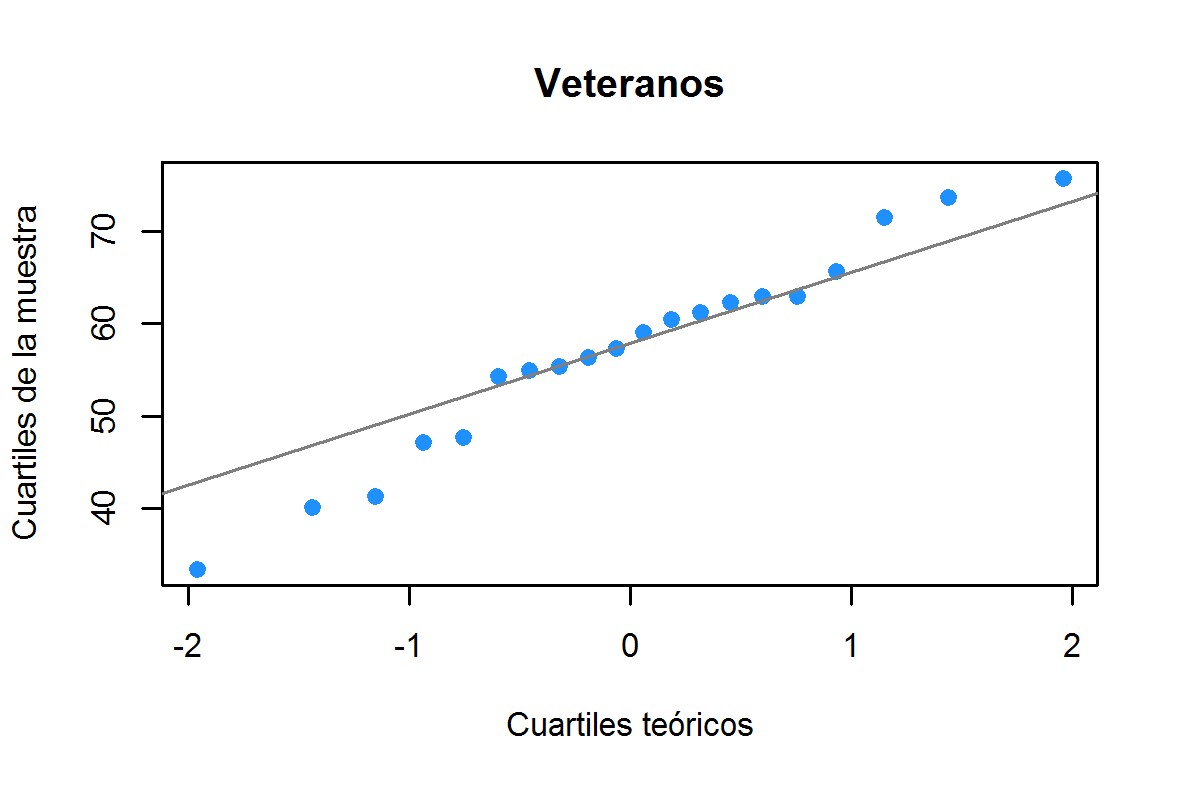
\includegraphics[scale=0.725]{./R/Graficos/CuartVeteranos.png}
\captionsetup{font={footnotesize,it}}
\caption{Diagramas de cuartiles para las categorías de la muestra.}
\label{fig:diagrama}
\end{figure}

Es interesante saber si la variable sexo tiene influencia sobre los tiempos obtenidos por los participantes de la prueba. Al ser el sexo de los participantes un factor de dos niveles, podemos realizar un contraste de hipótesis mediante un test de Welch. Obtenemos los resultados del cuadro \ref{tab:sexo} y la figura...... donde vemos que la media del tiempo empleado por las mujeres es casi 9 minutos superior al de los hombres. Además, un p-valor de 7,405e$^{-05}$ sugiere que la interpretación anterior de la diferencia de las medias es correcta. Realizando un análisis de varianza de un factor habríamos obtenido el mismo resultado.

\begin{table}[ht]
\centering
\begin{tabular}{cc}
\toprule[0.4mm]
Sexo & Tiempo empleado (minutos)\\
\midrule
Femenino & 59,93\\
Masculino & 50,96\\
\bottomrule[0.4mm]
\end{tabular}
\captionsetup{font={footnotesize,it}}
\caption{Resultados de las medias de tiempo por sexo de los participantes en la prueba.}
\label{tab:sexo}
\end{table}

Analizamos ahora la influencia que tienen los factores sexo y categoría sobre la variable tiempo en minutos. Primero analizamos la influencia de los dos factores por separado con una hipótesis nula (H$_{0}$) de que no afectan estos factores a los tiempos obtenidos por los participantes. Obtenemos los resultados del cuadro \ref{tab:anova1} donde vemos que ambos factores influyen por separado en los tiempos de la prueba deportiva.

\begin{table}[ht]
\centering
\begin{tabular}{cc}
\toprule[0.4mm]
Factor & Pr($>$F)\\
\midrule
Sexo & 2,09e$^{-05}$\\
Categoría & 0,0016\\
\bottomrule[0.4mm]
\end{tabular}
\captionsetup{font={footnotesize,it}}
\caption{Resultado del análisis de varianza para los factores sexo y categoría.}
\label{tab:anova1}
\end{table}

Una vez analizados por separado procedemos a hacerlo conjuntamente. En este caso el resultado que nos da es que conjuntamente no afectan al tiempo total de los participantes. Con un Pr($>$F) obtenido de 0,2478 aceptamos la H$_{0}$.

\end{document}